\documentclass[onecolumn,conference]{IEEEtran}
\IEEEoverridecommandlockouts
% The preceding line is only needed to identify funding in the first footnote. If that is unneeded, please comment it out.
\usepackage{cite}
\usepackage{amsmath,amssymb,amsfonts}
\usepackage{algorithmic}
\usepackage{graphicx}
\usepackage{textcomp}
\usepackage{xcolor}
\usepackage[linktocpage=true,colorlinks,citecolor=blue,pagebackref=true]{hyperref}
\usepackage{datetime}

\def\BibTeX{{\rm B\kern-.05em{\sc i\kern-.025em b}\kern-.08em
T\kern-.1667em\lower.7ex\hbox{E}\kern-.125emX}}

\begin{document}

    \title{A Framework for Survivability Evaluation}
    \IEEEpubid{$3^{rd}$ International Conference on
    Advanced Management Science, Kuala Lumpur, Malaysia, November 4-6 2011}
    \date{4 November 2011}

    \author{
    \IEEEauthorblockN{1\textsuperscript{st} Bahareh Abbasi}
    \IEEEauthorblockA{\textit{Department of Computer Engineering} \\
    \textit{Sharif University of Technology}\\
    Tehran, Iran \\
    b\_abbasi@alum.sharif.edu}
    \and
    \IEEEauthorblockN{2\textsuperscript{nd} Vahid Mavaji}
    \IEEEauthorblockA{\textit{Department of Computer Engineering} \\
    \textit{Sharif University of Technology}\\
    Tehran, Iran \\
    mavaji@alum.sharif.edu}
    }

    \maketitle

    \begin{abstract}
        Survivability is defined as the ability of a system to continue or to deliver its services to the users in presence of attacks, failures or accidents. After occurrence of failure, the system may work in the degraded and still acceptable level of performance states. So we have to extend the classical framework of reliability and fault tolerant mechanisms to systems which have to survive to failures or attacks (``failure tolerance''). The concept of graceful degradation is embedded in the notion of survivability though the system may stop working in presence of failure, and even enter the ``halt state''. In this paper, we present a paradigm that integrates the concept of survivability with the well-defined aspects of dependability by extending the fault-error-failure chain of dependable systems. We present our proposed framework using a sample packet switched network.
    \end{abstract}

    \begin{IEEEkeywords}
        Dependability, Survivability, Fault, Error, Failure, Halt
    \end{IEEEkeywords}

    \section{Introduction} \label{sec:intro}

    \section{Survivability and Related Concepts} \label{sec:rlwork}


    \section{A Framework for Survivability Evaluation} \label{sec:fram}

    \begin{figure}[htbp]
        \centering
        \makebox[\textwidth]{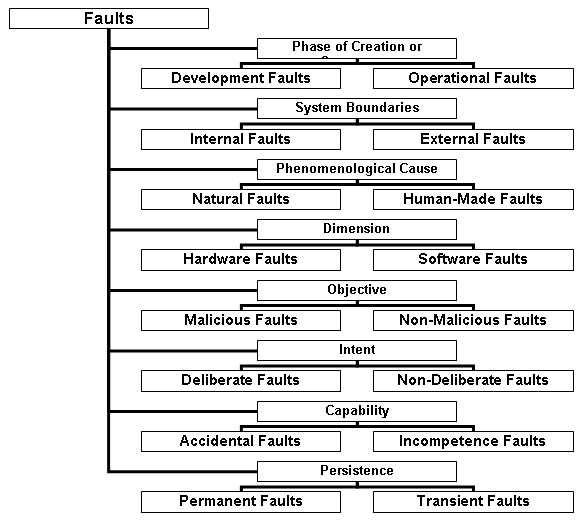
\includegraphics{icams1.png}}
        \caption{Elementary fault classes (redrawn from~\cite{b1})}
        \label{fig:1}
    \end{figure}


    \begin{figure}[htbp]
        \centering
        \makebox[\textwidth]{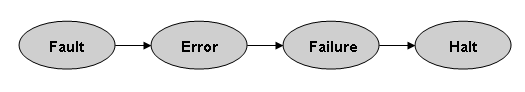
\includegraphics{icams2.png}}
        \caption{Cause-and-effect chain of dependability}
        \label{fig:2}
    \end{figure}




    \begin{figure}[htbp]
        \centering
        \makebox[\textwidth]{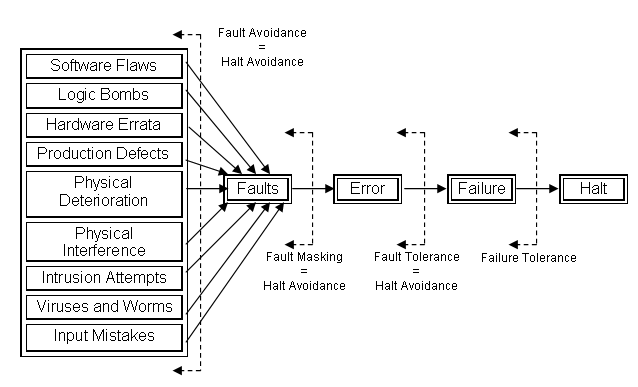
\includegraphics{icams3.png}}
        \caption{Relationship between fault-tolerance and survivability}
        \label{fig:3}
    \end{figure}



    \begin{figure}[htbp]
        \centering
        \makebox[\textwidth]{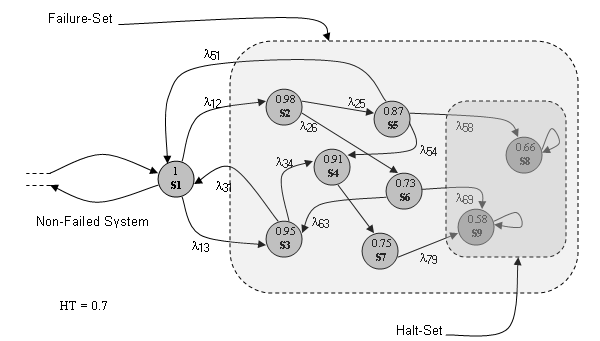
\includegraphics{icams4.png}}
        \caption{Different states after failure}
        \label{fig:4}
    \end{figure}



    \section{Conclusion} \label{sec:conc}
   
   
    \begin{thebibliography}{00}
        \bibitem{b1} A. Avizienis, J.C. Laprie, B. Randell, and C. Landwehr. Basic Concepts and Taxonomy of Dependable and Secure Computing. IEEE Transactions on Dependable and Secure Computing. 2004, 1(1).

        \bibitem{b2} G. Bolch, S. Greiner, H. Meer, K.S. Trivedi. Queuing Networks and Markov Chains Modeling and Performance Evaluation with Computer Science Applications.  John Wiley \& Sons, 1998.

        \bibitem{b3} I. Byon. Survivability of the U.S. Electric Power Industry. Master thesis, Carnegie Mellon University Pittsburgh, Pennsylvania, May 2000.

        \bibitem{b4} J. Caldera. Survivability Requirements for the U.S. Healthcare Industry. Master thesis, Carnegie Mellon University Pittsburgh, Pennsylvania, May 2000.

        \bibitem{b5} R.J. Ellison, D.A. Fisher, R.C. Linger, H.F. Lipson, T.A. Longstaff and N.R. Mead. An Approach to Survivable Systems. NATO IST Symposium on Protecting Information Systems in the 21st Century. 1999.

        \bibitem{b6} R.J. Ellison, R.C. Linger, H.F. Lipson, T.A. Longstaff and N.R. Mead. A Case study in Requirements for Survivable Systems. SEI. 2002.

        \bibitem{b7} H. Frank. Survivability analysis of command and control communications networks-part I\&II. IEEE Transactions on Communications. 1974, 22(5): 589-605.

        \bibitem{b8} M. Keshtgary. General Framework for networksurvivability performance evaluation.  Ph.D. Dissertation, Sharif University of Technology, Dept. of Computer Eng, Tehran, Iran. 2005.

        \bibitem{b9} M. Keshtgary, F. Al-Zahrani, A. P. Jayasumana  and A.H. Jahangir. Network Survivability Performance Evaluation with Applications in WDM Networks with Wavelength Conversion.  Proc. Of 29th IEEE Conference on Local Computer Networks. 2004, pp. 344-351.

        \bibitem{b10} J.C. Knight, E. A. Strunk, K J. Sullivan . Towards a Rigorous Definition of Information System Survivability. Darpa Information survivability Conference and Exposition. Volume 1. 2003.

        \bibitem{b11} K. Kyamakya, K. Jobman, M. Meincke. Security and Survivability of Distributed Systems: An Overview. Proc. Of 21st Century Military Communications Conference, Volume 1, IEEE. 2000, pp. 1204-1208.

        \bibitem{b12} S.C. Liew and K.W. Lu. A framework for characterizing disaster-based network survivability.  IEEE Journal on Selected Areas in Communications. 1994, 12(1): 52-58.

        \bibitem{b13} H. Shrobe. Model-Based Troubleshooting for Information Survivability.  DARPA Information Survivability Conference and Exposition, Volume 2, IEEE. 1999, pp. 231-240.

        \bibitem{b14} J.M. Voas, A.K. Ghosh. Software Fault Injection for Survivability. DARPA Information Survivability Conference and Exposition. Volume 2, IEEE. 1999, pp. 256-270.

        \bibitem{b15} C. Wang, J. Davidson, J. Hill, J. Knight. Protection of Software-Based Survivability Mechanisms.  the International Conference on Dependable Systems and Networks, IEEE. 2001, pp. 1413-1420.

        \bibitem{b16} M. Wilikens, T. Jackson. Survivability of Networked Information Systems and Infrastructures.  European Commission Directorate.

        \bibitem{b17} R. Wolff. Poisson arrivals see time averages. Operations Research, 30. 1982, pp. 223-231.

        \bibitem{b18} A. Zolfaghari and F.J. Kaudel. Framework for network survivability performance.  IEEE Journal on Selected Areas in Communications. 1994, 12(1): 46-51.

    \end{thebibliography}
\end{document}
